%%%%%%%%%%%%%%%%%%%%%%%%%%%%%%%%%%%%%%%%%%%%%%%%%%%%%%%%%%%%%%%%%%%%%%%%
%% Customizações do abnTeX2 (http://abnTeX2.googlecode.com)           %%
%% para a Universidade Estadual do Ceara - UECE                       %%
%%                                                                    %%
%% This work may be distributed and/or modified under the             %% 
%% conditions of the LaTeX Project Public License, either version 1.3 %%
%% of this license or (at your option) any later version.             %%
%% The latest version of this license is in                           %%
%%   http://www.latex-project.org/lppl.txt                            %%
%% and version 1.3 or later is part of all distributions of LaTeX     %%
%% version 2005/12/01 or later.                                       %%
%%                                                                    %%
%% This work has the LPPL maintenance status `maintained'.            %%
%%                                                                    %%
%% The Current Maintainer of this work is Thiago Nascimento           %%
%%                                                                    %%
%% Project available on: https://github.com/thiagodnf/uecetex2        %%
%%                                                                    %%
%% Further information about abnTeX2                                  %%
%% are available on http://abntex2.googlecode.com/                    %%
%%                                                                    %%
%%%%%%%%%%%%%%%%%%%%%%%%%%%%%%%%%%%%%%%%%%%%%%%%%%%%%%%%%%%%%%%%%%%%%%%%

%%%%%%%%%%%%%%%%%%%%%%%%%%%%%%%%%%%%%%%%%%%%%%%%%%%%%%%%%%%%%%%%%%%%%%%%
%% Customizações do abnTeX2 (http://abnTeX2.googlecode.com)           %%
%% para a Universidade Estadual do Ceara - UECE                       %%
%%                                                                    %%
%% This work may be distributed and/or modified under the             %% 
%% conditions of the LaTeX Project Public License, either version 1.3 %%
%% of this license or (at your option) any later version.             %%
%% The latest version of this license is in                           %%
%%   http://www.latex-project.org/lppl.txt                            %%
%% and version 1.3 or later is part of all distributions of LaTeX     %%
%% version 2005/12/01 or later.                                       %%
%%                                                                    %%
%% This work has the LPPL maintenance status `maintained'.            %%
%%                                                                    %%
%% The Current Maintainer of this work is Thiago Nascimento           %%
%%                                                                    %%
%% Project available on: https://github.com/thiagodnf/uecetex2        %%
%%                                                                    %%
%% Further information about abnTeX2                                  %%
%% are available on http://abntex2.googlecode.com/                    %%
%%                                                                    %%
%%%%%%%%%%%%%%%%%%%%%%%%%%%%%%%%%%%%%%%%%%%%%%%%%%%%%%%%%%%%%%%%%%%%%%%%

\documentclass[        
    a4paper,          % Tamanho da folha A4
    12pt,             % Tamanho da fonte 12pt
    chapter=TITLE,    % Todos os capitulos devem ter caixa alta
    section=TITLE,    % Todas as secoes devem ter caixa alta
    oneside,          % Usada para impressao em apenas uma face do papel
    english,          % Hifenizacoes em ingles
    spanish,          % Hifenizacoes em espanhol
    brazil            % Ultimo idioma eh o idioma padrao do documento
]{abntex2}


% Importações de pacotes
\usepackage[utf8]{inputenc}                         % Acentuação direta
\usepackage[T1]{fontenc}                            % Codificação da fonte em 8 bits
\usepackage{graphicx}                               % Inserir figuras
\usepackage{amsfonts, amssymb, amsmath}             % Fonte e símbolos matemáticos
\usepackage{booktabs}                               % Comandos para tabelas
\usepackage{verbatim}                               % Texto é interpretado como escrito no documento
\usepackage{multirow, array}                        % Múltiplas linhas e colunas em tabelas
\usepackage{indentfirst}                            % Endenta o primeiro parágrafo de cada seção.
\usepackage{microtype}                              % Para melhorias de justificação?
\usepackage[portuguese,ruled,lined]{algorithm2e}    % Escrever algoritmos
\usepackage{algorithmic}                            % Criar Algoritmos  
%\usepackage{float}                                  % Utilizado para criação de floats
\usepackage{amsgen}
\usepackage{lipsum}                                 % Usar a simulação de texto Lorem Ipsum
%\usepackage{titlesec}                               % Permite alterar os títulos do documento
\usepackage{tocloft}                                % Permite alterar a formatação do Sumário
\usepackage{etoolbox}                               % Usado para alterar a fonte da Section no Sumário
\usepackage[nogroupskip,nonumberlist,acronym]{glossaries}                % Permite fazer o glossario
\usepackage{caption}                                % Altera o comportamento da tag caption,nb          
\usepackage[alf, abnt-emphasize=bf, bibjustif, recuo=0cm, abnt-etal-cite=2, abnt-etal-list=0]{abntex2cite}  % Citações padrão ABNT
%\usepackage[bottom]{footmisc}                      % Mantém as notas de rodapé sempre na mesma posição
\usepackage{helvet}
\renewcommand{\familydefault}{\sfdefault}                                % Usa a fonte Arial
\usepackage{mathptmx}                               % Usa a fonte Times New Roman										
%\usepackage{lmodern}                               % Usa a fonte Latin Modern
%\usepackage{subfig}                                % Posicionamento de figuras
%\usepackage{scalefnt}                              % Permite redimensionar tamanho da fonte
%\usepackage{color, colortbl}                       % Comandos de cores
%\usepackage{lscape}                                % Permite páginas em modo "paisagem"
%\usepackage{ae, aecompl}                           % Fontes de alta qualidade
%\usepackage{picinpar}                              % Dispor imagens em parágrafos
%\usepackage{latexsym}                              % Símbolos matemáticos
%\usepackage{upgreek}                               % Fonte letras gregas
\usepackage{appendix}                               % Gerar o apendice no final do documento
\usepackage{paracol}                                % Criar paragrafos sem identacao
\usepackage{lib/uecetex2}		                    % Biblioteca com as normas da UECE para trabalhos academicos
\usepackage{pdfpages}                               % Incluir pdf no documento
\usepackage{amsmath}                                % Usar equacoes matematicas
\usepackage{colortbl}
% Organiza e gera a lista de abreviaturas, simbolos e glossario
\makeglossaries

% Gera o Indice do documento
\makeindex


%%%%%%%%%%%%%%%%%%%%%%%%%%%%%%%%%%%%%%%%%%%%%%%%%%%%%
%%          Configuracoes do ueceTeX2              %%
%%%%%%%%%%%%%%%%%%%%%%%%%%%%%%%%%%%%%%%%%%%%%%%%%%%%%

% Opcoes disponiveis

\trabalhoacademico{tccgraduacao}
%\trabalhoacademico{tccespecializacao}
%\trabalhoacademico{dissertacao}
%\trabalhoacademico{tese}

% Define se o trabalho eh uma qualificacao
% Coloque 'nao' para versao final do trabalho

\ehqualificacao{nao}

% Remove as bordas vermelhas e verdes do PDF gerado
% Coloque 'sim' pare remover

\removerbordasdohyperlink{sim} 

% Adiciona a cor Azul a todos os hyperlinks

\cordohyperlink{nao}

%%%%%%%%%%%%%%%%%%%%%%%%%%%%%%%%%%%%%%%%%%%%%%%%%%%%%
%%          Informação sobre a IES                 %%
%%%%%%%%%%%%%%%%%%%%%%%%%%%%%%%%%%%%%%%%%%%%%%%%%%%%%

\ies{Universidade de São Paulo}
\iessigla{USP}
\centro{Instituto de Ciências Matemáticas e de Computação}

%%%%%%%%%%%%%%%%%%%%%%%%%%%%%%%%%%%%%%%%%%%%%%%%%%%%%
%%        Informação para TCC de Graduacao         %%
%%%%%%%%%%%%%%%%%%%%%%%%%%%%%%%%%%%%%%%%%%%%%%%%%%%%%

\graduacaoem{Sistema de Informação}
\habilitacao{bacharel} % Pode colocar tambem 'licenciada'

%%%%%%%%%%%%%%%%%%%%%%%%%%%%%%%%%%%%%%%%%%%%%%%%%%%%%
%%     Informação para TCC de Especializacao       %%
%%%%%%%%%%%%%%%%%%%%%%%%%%%%%%%%%%%%%%%%%%%%%%%%%%%%%

\especializacaoem{}

%%%%%%%%%%%%%%%%%%%%%%%%%%%%%%%%%%%%%%%%%%%%%%%%%%%%%
%%         Informação para Dissertacao             %%
%%%%%%%%%%%%%%%%%%%%%%%%%%%%%%%%%%%%%%%%%%%%%%%%%%%%%

\programamestrado{Programa de Pós-Graduação em Ciência da Computação}
\nomedomestrado{Mestrado Acadêmico em Ciência da Computação}
\mestreem{Ciência da Computação}
\areadeconcentracaomestrado{Ciência da Computação}

%%%%%%%%%%%%%%%%%%%%%%%%%%%%%%%%%%%%%%%%%%%%%%%%%%%%%
%%               Informação para Tese              %%
%%%%%%%%%%%%%%%%%%%%%%%%%%%%%%%%%%%%%%%%%%%%%%%%%%%%%

\programadoutorado{Programa de Pós-Graduação em Saúde Coletiva}
\nomedodoutorado{Doutorado em Saúde Coletiva}
\doutorem{Saúde Coletiva}
\areadeconcentracaodoutorado{Saúde Coletiva}

%%%%%%%%%%%%%%%%%%%%%%%%%%%%%%%%%%%%%%%%%%%%%%
%%  Informação relacionadas ao trabalho     %%
%%%%%%%%%%%%%%%%%%%%%%%%%%%%%%%%%%%%%%%%%%%%%%

\autor{Leandro Satoshi de Siqueira\\
Gabriel Silva Fontes}
\titulo{Árvore de busca binária}
\data{2018}
\local{São Carlos - São Paulo}

% Exemplo: \dataaprovacao{01 de Janeiro de 2012}
\dataaprovacao{}

%%%%%%%%%%%%%%%%%%%%%%%%%%%%%%%%%%%%%%%%%%%%%
%%     Informação sobre o Orientador       %%
%%%%%%%%%%%%%%%%%%%%%%%%%%%%%%%%%%%%%%%%%%%%%

\orientador{Adenilso da Silva Simão}
\orientadories{Universidade de São Paulo - USP}
\orientadorcentro{Instituto de Ciências Matemáticas e de Computação  - ICMC}
\orientadorfeminino{} % Coloque 'sim' se for do sexo feminino

%%%%%%%%%%%%%%%%%%%%%%%%%%%%%%%%%%%%%%%%%%%%%
%%      Informação sobre o Co-orientador   %%
%%%%%%%%%%%%%%%%%%%%%%%%%%%%%%%%%%%%%%%%%%%%%

% Deixe o nome do coorientador em branco para remover do documento

\coorientador{}
\coorientadories{Universidade Co-orientador - SIGLA}
\coorientadorcentro{Centro do Co-orientador - SIGLA}
\coorientadorfeminino{nao} % Coloque 'sim' se for do sexo feminino

%%%%%%%%%%%%%%%%%%%%%%%%%%%%%%%%%%%%%%%%%%%%%
%%      Informação sobre a banca           %%
%%%%%%%%%%%%%%%%%%%%%%%%%%%%%%%%%%%%%%%%%%%%%

% Atenção! Deixe o nome do membro da banca para remover da folha de aprovacao

% Exemplo de uso:
% \membrodabancadois{Prof. Dr. Fulano de Tal}
% \membrodabancadoisies{Universidade Estadual do Ceará - UECE}

\membrodabancadois{Membro da Banca Dois}
\membrodabancadoiscentro{Faculdade de Filosofia Dom Aureliano Matos – FAFIDAM}
\membrodabancadoisies{Universidade do Membro da Banca Dois - SIGLA}
\membrodabancatres{Membro da Banca Três}
\membrodabancatrescentro{Centro de Ciências e Tecnologia - CCT}
\membrodabancatresies{Universidade do Membro da Banca Três - SIGLA}
\membrodabancaquatro{Membro da Banca Quatro}
\membrodabancaquatrocentro{Centro de Ciências e Tecnologia - CCT}
\membrodabancaquatroies{Universidade do Membro da Banca Quatro - SIGLA}
\membrodabancacinco{Membro da Banca Cinco}
\membrodabancacincocentro{Teste}
\membrodabancacincoies{Universidade do Membro da Banca Cinco - SIGLA}
\membrodabancaseis{Membro da Banca Seis}
\membrodabancaseiscentro{}
\membrodabancaseisies{Universidade do Membro da Banca Seis - SIGLA}



\begin{document}	

	% Elementos pré-textuais
	\imprimircapa
	\imprimirfolhaderosto{}
	%\imprimirfichacatalografica{elementos-pre-textuais/ficha-catalografica}
	%\imprimirerrata{elementos-pre-textuais/errata}
	%\imprimirfolhadeaprovacao
	%\imprimirdedicatoria{elementos-pre-textuais/dedicatoria}
	%\imprimiragradecimentos{elementos-pre-textuais/agradecimentos}
	%\imprimirepigrafe{Charles Chaplin}{elementos-pre-textuais/epigrafe}
	%\imprimirresumo{elementos-pre-textuais/resumo}
	%\imprimirabstract{elementos-pre-textuais/abstract}
	%\imprimirlistadeilustracoes
	%\imprimirlistadetabelas
	%\imprimirlistadequadros
	%\imprimirlistadealgoritmos
	%\imprimirlistadeabreviaturasesiglas	
	%\imprimirlistadesimbolos{elementos-pre-textuais/lista-de-simbolos}   
	\imprimirsumario
	
	%Elementos textuais
	\textual
	\chapter{Introdução}
\label{cap:introducao}
Este trabalho refere-se à implementação da árvore de busca binária e suas funções estudadas nas aulas da disciplina de Introdução à ciência de computação II.

Primeiramente será feita uma análise de suas funcionalidades e gastos de tempo e memória para os mesmos, e em seguida algumas discussões em relação a implementação e resultados obtidos.


	\chapter{Metodologia}
\label{chap:metodologia}

A metodologia utilizada foi um estudo prévio da estrutura de dados e suas funcionalidades, seguido de sua implementação e de testes práticos para validação dos resultados anteriormente obtidos.
Serão avaliados os gastos para armazenamento, inserção, remoção e busca de elementos.

Como um complemento ao acima avaliado, será analisado também uma otimização da árvore de busca binária, a árvore AVL e o algoritmo de rotação para balanceamento da mesma.\\
	\chapter{A Estrutura}
\label{cap:estrutura}

\section{Definição}
\label{sec:definicao}
uma árvore binária de busca (ou árvore binária de pesquisa) é uma estrutura de dados de árvore binária baseada em nós, onde todos os nós da subárvore esquerda possuem um valor numérico inferior ao nó raiz e todos os nós da subárvore direita possuem um valor superior ao nó raiz.
\cite{ABBwiki}

\section{Elementos e Terminologias}
\label{sec:elementos}
\begin{itemize}
    \item Nós - são todos os itens guardados na árvore
    \item Raiz - é o nó do topo da árvore 
    \item Filhos - são os nós que vem depois dos outros nós 
    \item Pais - são os nós que vem antes dos outros nós 
    \item Folhas - são os nós que não têm filhos; são os últimos nós da árvore
    \item Grau - número de sub-árvores relacionadas àquele nó.  
    \item Altura - comprimento do caminho mais longo do nó a uma folha 
    \item Profundidade - comprimento do unico caminho entre o nó raiz e o nó avaliado
\end{itemize}
	\chapter{Discussões e Resultados}
\label{chap:discussoes e resultados}

A árvore de busca binária é uma estrutura de dados focada em armazenar elementos de forma ordenada afim de agilizar o máximo possivel a tarefa de busca.
Contudo, para garantir essa melhora na eficiencia são necessários alguns pré-requisitos, além de dificultar de certa forma outras operações.

O ideal para uma árvore binária é garantir um tempo de O($n\log(n)$) ou algo próximo disso, e para isso é preciso uma árvore o mais balanceada possivel, isto é,

Ao inserir elementos na árvore deve-se tomar cuidado com o elemento inicial e na ordenação relativa desses, pois pode-se facilmente degenerar a estrutura da árvore para uma lista, ou algo próximo disso, acabando completamente com seu propósito.

O armazenamento na árvore binária tem um custo semelhante a uma lista dinâmica encadeada, ocupando um espaço maior do que uma lista estática comum, porém com a vantagem de não ocupar espaço desnecessário e poder aumenta a lista a qualquer momento.

A inserção tem um custo baixo, devido a organização com ponteiros, é necessario apenas uma atribuição após encontrar o lugar, garantindo algo próximo de O($\log(n)$, como será explicado a mais a frente.

A remoção nessa estrutura, apesar de não tem um custo alto, tem uma grande complexidade e pode acabar com o balanceamento da árvore, prejudicando assim todas as outras funcionalidades.

A busca na árvore pode ser realizada como se estivesse em uma lista estatica ordenada realizando uma busca binária, porém ocorre de forma ainda mais direta, devido sua organização. Por conta disso é quase sempre sempre possivel conseguir um tempo O($\log(n))$, porém, assim como todas operações, isso depende do balanceamento.

Uma árvore AVL é uma árvore binária de busca balanceada, e isso implica que a diferença na altura das duas sub-árvores filhas diferir em módulo de até uma unidade. Garantindo uma árvore ser AVL, garante-se uma altura de $\log(n)$ e também um custo de O($\log(n)$) para busca inserção e remoção.

Um metodo utilizado para garantir o balanceamento é um algoritmo de rotação executado conforme a necessidade após operações de remoção ou inserção. De forma superficial, existem quatro tipos de rotações, à direita ou à esquerda, e simples ou dupla, que quando executados em conjunto, literalmente rotacionam uma sub-árvore para balancea-la.
	%\chapter{Trabalhos Relacionados}
\label{cap:trabalhos-relacionados}

Integer non lacinia magna. Aenean tempor lorem tellus, non sodales nisl commodo ut. Proin mattis placerat risus sit amet laoreet. Praesent sapien arcu, maximus ac fringilla efficitur, vulputate faucibus sem. Donec aliquet velit eros, sit amet elementum dolor pharetra eget. Integer eget mattis libero

\section{Trabalho Relacionado A}
\label{sec:trabalho-relacionado-a}

\lipsum[10]

	\begin{figure}[h!]
		\centering
		\Caption{\label{fig:exemplo-1} Lorem ipsum dolor sit amet, consectetur adipiscing elit. Suspendisse commodo lectus et augue elementum varius.}	
		\UECEfig{}{
			\fbox{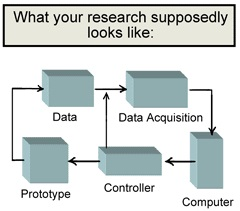
\includegraphics[width=8cm]{figuras/figura-1}}
		}{
			\Fonte{Elaborado pelo autor}
		}	
	\end{figure}
	
\lipsum[11]

\section{Trabalho Relacionado B}
\label{sec:trabalho-relacionado-b}

Integer non lacinia magna. Aenean tempor lorem tellus, non sodales nisl commodo ut. Proin mattis placerat risus sit amet laoreet. Praesent sapien arcu, maximus ac fringilla efficitur, vulputate faucibus sem. Donec aliquet velit eros, sit amet elementum dolor pharetra eget. Integer eget mattis libero. Praesent ex velit, pulvinar at massa vel, fermentum dictum mauris. Ut feugiat accumsan augue, et ultrices ipsum euismod vitae

	\begin{figure}[h!]
		\centering
		\Caption{\label{fig:exemplo-2} Maecenas luctus augue odio, sed tincidunt nunc posuere nec}	
		\UECEfig{}{
			\fbox{
\includegraphics[width=8cm]{figuras/figura-2}}
		}{
			\Fonte{Elaborado pelo autor}			
		}	
	\end{figure}

Nunc ac pretium dui. Mauris aliquam dapibus nulla ac mattis. Aenean non tortor volutpat, varius lectus vitae, accumsan nibh. Cras pretium vestibulum enim, id ullamcorper tortor ultrices non. Integer sodales viverra faucibus. Curabitur at dui lacinia, rhoncus lacus at, blandit metus. Integer scelerisque non enim quis ornare.

	\begin{quadro}[h!]	
		\centering
		\Caption{\label{qua:exemplo-1} Praesent ex velit, pulvinar at massa vel, fermentum dictum mauris. Ut feugiat accumsan augue}		
		\UECEqua{}{
			\begin{tabular}{|c|c|l|l|}
				\hline
				Quisque & pharetra & tempus & vulputate \\
				\hline
				E1 & Complete coverage by a single transcript & Both  & Complete\\
				\hline
				E2 & Complete coverage by more than & Both splice sites & Complete\\
				\hline
				E3 & Partial coverage & Both splice sites & Both \\				
				\hline
			\end{tabular}
		}{
			\Fonte{Elaborado pelo autor}
		}
	\end{quadro}
	
\lipsum[20]

	
	\begin{quadro}[h!]	
		\centering
		\Caption{\label{qua:exemplo-2} Duis faucibus, enim quis tincidunt pellentesque}		
		\UECEqua{}{
			\begin{tabular}{|c|c|}
				\hline
				Quisque & pharetra \\
				\hline
				E1 & Complete coverage by a single transcript \\
				\hline
				E2 & Complete coverage by more than \\
				\hline
				E3 & Partial coverage \\
				\hline
				E4 & Partial coverage \\
				\hline
				E5 & Partial coverage \\
				\hline
				E6 & Partial coverage \\
				\hline
				E7 & Partial coverage \\
				\hline
			\end{tabular}
		}{
			\Fonte{Elaborado pelo autor}
		}
	\end{quadro}

\lipsum[21]

Integer non lacinia magna. Aenean tempor lorem tellus, non sodales nisl commodo ut. Proin mattis placerat risus sit amet laoreet. Praesent sapien arcu, maximus ac fringilla efficitur, vulputate faucibus sem. Donec aliquet velit eros, sit amet elementum dolor pharetra eget. Integer eget mattis libero.
\Gls{ambiguidade}
\Gls{braile}
\Gls{coerencia}
\Gls{dialetos}
\Gls{elipse}
\Gls{locucao-adjetiva}
\Gls{modificadores}
\Gls{paronimos}
\Gls{sintese}
\Gls{borboleta}
	%\chapter{Exemplo de Capítulos e Seções}
\label{chap:exemplo-de-capitulos-e-secoes}

Este capítulo descreve como você deve formatar os títulos do seu trabalho, ensinando também como você deve usá-los. O capítulo deve ser caixa alta, 12pt e com negrito. Para fazer um capítulo, você deve fazer:

\verb!\chapter{Escreva aqui o nome do Capítulo}!

\section{Seção Secundária}
As seções Secundárias deve ser caixa alta, 12pt e sem negrito. Para fazer uma seção Secundária, você deve fazer:

\verb!\section{Escreva aqui o nome da seção}!

\subsection{Seção Terciária}
As seções Terciárias deve ser caixa alta e baixa, 12pt e com negrito. Para fazer uma seção Terciária, você deve fazer:

\verb!\subsection{Escreva aqui o nome da seção}!

\subsubsection{Seção Quaternária}
As seções Quaternárias deve ser caixa alta e baixa, 12pt e sem negrito. Para fazer uma seção Quaternária, você deve fazer:

\verb!\subsubsection{Escreva aqui o nome da seção}!

\subsubsubsection{Seção Quinária}
As seções Quinárias deve ser caixa alta e baixa, 12pt e com itálico. Para fazer uma seção Quinária, você deve fazer:

\verb!\subsubsubsection{Escreva aqui o nome da seção}!
	%\chapter{Conclusão}
\label{chap:conclusao}

	%\chapter{CRONOGRAMA}
\label{ap:modelo-de-capa}

\center

\begin{enumerate}
\item Pesquisa bibliográfica
\item Estudo e preparação do estado da arte
\item Programação e/ou experimentação e/ou simulação
\item Análise dos resultados
\item Redação da dissertação
\item Apresentação do trabalho
\end{enumerate}

\begin{table}[h]
	\centering
	\begin{tabular}{|l|l|l|l|l|}
	\hline
	\multicolumn{1}{|c|}{} &
	\multicolumn{4}{|c|}{MESES} \\
	\hline
	\multicolumn{1}{|c|}{ETAPAS} &
	\multicolumn{1}{c|}{Mês 1} &
	\multicolumn{1}{c|}{Mês 2} &
	\multicolumn{1}{c|}{Mês 3} &
	\multicolumn{1}{c|}{Mês 4} \\
	\hline
        \multicolumn{1}{|c|}{1} &
        \cellcolor[gray]{0.8}\color{black} &
        \multicolumn{1}{c|}{} &
        \multicolumn{1}{c|}{} &
        \multicolumn{1}{c|}{} \\
	\hline
        \multicolumn{1}{|c|}{2} &
        \cellcolor[gray]{0.8}\color{black} &
        \multicolumn{1}{c|}{} &
        \multicolumn{1}{c|}{} &
        \multicolumn{1}{c|}{} \\
	\hline
        \multicolumn{1}{|c|}{3} &
        \multicolumn{1}{c|}{} &
        \cellcolor[gray]{0.8}\color{black} &
        \multicolumn{1}{c|}{} &
        \multicolumn{1}{c|}{} \\
	\hline
        \multicolumn{1}{|c|}{4} &
        \multicolumn{1}{c|}{} &
        \multicolumn{1}{c|}{} &
        \cellcolor[gray]{0.8}\color{black} &
        \multicolumn{1}{c|}{} \\
	\hline
        \multicolumn{1}{|c|}{5} &
        \multicolumn{1}{c|}{} &
        \multicolumn{1}{c|}{} &
        \multicolumn{1}{c|}{} &
        \cellcolor[gray]{0.8}\color{black} \\
	\hline
        \multicolumn{1}{|c|}{6} &
        \multicolumn{1}{c|}{} &
        \multicolumn{1}{c|}{} &
        \multicolumn{1}{c|}{} &
        \cellcolor[gray]{0.8}\color{black} \\
%	\hline
%        \multicolumn{1}{|c|}{7} &
%        \multicolumn{1}{c|}{} &
%        \multicolumn{1}{c|}{} &
%        \multicolumn{1}{c|}{} &
%        \multicolumn{1}{c|}{} \\
	\hline
	\end{tabular}
\end{table}
	
	%Elementos pós-textuais	
	\bibliography{elementos-pos-textuais/referencias}
	%\imprimirglossario	
	%\imprimirapendices
		% Adicione aqui os apendices do seu trabalho
		%\chapter{CRONOGRAMA}
\label{ap:modelo-de-capa}

\center

\begin{enumerate}
\item Pesquisa bibliográfica
\item Estudo e preparação do estado da arte
\item Programação e/ou experimentação e/ou simulação
\item Análise dos resultados
\item Redação da dissertação
\item Apresentação do trabalho
\end{enumerate}

\begin{table}[h]
	\centering
	\begin{tabular}{|l|l|l|l|l|}
	\hline
	\multicolumn{1}{|c|}{} &
	\multicolumn{4}{|c|}{MESES} \\
	\hline
	\multicolumn{1}{|c|}{ETAPAS} &
	\multicolumn{1}{c|}{Mês 1} &
	\multicolumn{1}{c|}{Mês 2} &
	\multicolumn{1}{c|}{Mês 3} &
	\multicolumn{1}{c|}{Mês 4} \\
	\hline
        \multicolumn{1}{|c|}{1} &
        \cellcolor[gray]{0.8}\color{black} &
        \multicolumn{1}{c|}{} &
        \multicolumn{1}{c|}{} &
        \multicolumn{1}{c|}{} \\
	\hline
        \multicolumn{1}{|c|}{2} &
        \cellcolor[gray]{0.8}\color{black} &
        \multicolumn{1}{c|}{} &
        \multicolumn{1}{c|}{} &
        \multicolumn{1}{c|}{} \\
	\hline
        \multicolumn{1}{|c|}{3} &
        \multicolumn{1}{c|}{} &
        \cellcolor[gray]{0.8}\color{black} &
        \multicolumn{1}{c|}{} &
        \multicolumn{1}{c|}{} \\
	\hline
        \multicolumn{1}{|c|}{4} &
        \multicolumn{1}{c|}{} &
        \multicolumn{1}{c|}{} &
        \cellcolor[gray]{0.8}\color{black} &
        \multicolumn{1}{c|}{} \\
	\hline
        \multicolumn{1}{|c|}{5} &
        \multicolumn{1}{c|}{} &
        \multicolumn{1}{c|}{} &
        \multicolumn{1}{c|}{} &
        \cellcolor[gray]{0.8}\color{black} \\
	\hline
        \multicolumn{1}{|c|}{6} &
        \multicolumn{1}{c|}{} &
        \multicolumn{1}{c|}{} &
        \multicolumn{1}{c|}{} &
        \cellcolor[gray]{0.8}\color{black} \\
%	\hline
%        \multicolumn{1}{|c|}{7} &
%        \multicolumn{1}{c|}{} &
%        \multicolumn{1}{c|}{} &
%        \multicolumn{1}{c|}{} &
%        \multicolumn{1}{c|}{} \\
	\hline
	\end{tabular}
\end{table}
		%\apendice{Modelo de Capa}
\label{ap:modelo-de-capa}

\lipsum[1]

		%\apendice{Termo de Fiel Depositário}
\label{ap:termo-de-fiel-depositario}

\noindent \textbf{Pesquisa:} ANÁLISE DA MORTALIDADE INFANTIL COM MALFORMAÇÕES CONGÊNITAS.

\noindent Pelo presente instrumento que atende às exigências legais, a Sra. Maria Consuelo Martins Saraiva, ``fiel depositário'' com o cargo de Secretária Municipal de Saúde de Iracema, após ter tomado conhecimento do protocolo de pesquisa intitulado: ANÁLISE DA MORTALIDADE INFANTIL COM MALFORMAÇÕES CONGÊNITAS. Analisando a repercussão desse estudo no contexto da saúde pública e epidemiologia, autoriza Karla Maria da Silva Lima, enfermeira, aluna do Curso de Mestrado Acadêmico em Enfermagem da Universidade Estadual do Ceará (UECE), sob orientação do Prof. Dr. José Maria de Castro, da UECE, ter acesso aos bancos de dados do Sistema de Informação sobre Nascidos Vivos e do Sistema de Informação sobre Mortalidade da Secretaria Municipal de Saúde de Iracema, objeto deste estudo, e que se encontram sob sua total responsabilidade. Fica claro que o Fiel Depositário pode a qualquer momento retirar sua AUTORIZAÇÃO e ciente de que todas as informações prestadas tornar-se-ão confidenciais e guardadas por força de sigilo profissional, assegurando que os dados obtidos da pesquisa serão somente utilizados para estudo.	
	%\imprimiranexos
		% Adicione aqui os anexos do seu trabalho
		%\anexo{Dinâmica das classes sociais}
\label{an:dinamica-das-classes-sociais}

\index{AAA}
	%\imprimirindice

\end{document}